\chapter{Spremenljivost podatkovnih tipov in terke}

\section{Kaj je spremenljivost?}

Določeni podatkovni tipi v Pythonu so spremenljivi \angl{mutable}, določeni pa ne. Kaj to pomeni? Če je nek podatek nespremenljiv \angl{immutable}, to pomeni, da ga po tistem, ko je enkrat ustvarjen, ne moremo več spreminjati. Lahko pa naredimo nov podatek, ki odraža spremembo, ki jo želimo nad podatkom narediti. Primeri nespremenljivih podatkovnih tipov so števila tipa \texttt{int} in \texttt{float}, niz oziroma \texttt{str} in \texttt{bool} (spremenljivost osnovnih podatkovnih tipov v jeziku Python prikazuje tabela \ref{tab:spremenljivost}). To so torej skoraj vsi podatkovni tipi, ki smo jih do sedaj spoznali. Če je določen podatek spremenljiv, potem ga lahko spreminjamo tudi kasneje. Primer spremenljivega podatkovnega tipa je seznam oziroma \texttt{list}. Spremenljivost podatkovnih tipov na videz izgleda kot nekaj, s čimer se nam pri osnovah programiranja niti ne bi bilo potrebno ukvarjati. Žal pa ima veliko posledic, ki jih brez razumevanja spremenljivosti težko razumemo, zato je smiselno, da si celoten koncept podrobneje pogledamo. 
\begin{table}
    \caption{Spremenljivost osnovnih podatkovnih tipov v jeziku Python}
    \label{tab:spremenljivost}
    \centering
    \begin{tabular}{c|c|c}
    podatkovni tip & opis & spremenljiv  \\
    \hline
    \texttt{bool}& \textit{boolean} (\texttt{True, False}) & Ne \\
    \texttt{int}& \textit{integer} (celo število) & Ne \\
    \texttt{float}& \textit{floating-point} (decimalno število) & Ne \\
    \texttt{str}& \textit{string} (niz) & Ne \\
    \texttt{list}& \textit{list} (seznam) & Da \\
    \texttt{tuple}& \textit{tuple} (terka) & Ne \\
    \texttt{dict}& \textit{dictionary} (slovar) & Da \\
    \texttt{set}& \textit{set} (množica) & Da \\
    \texttt{frozenset}& \textit{frozenset} (nespremenljiva množica) & Ne \\
    \end{tabular}
\end{table}

\section{Kaj se zgodi ob prirejanju spremenljivk?}
Kaj se zgodi, ko spremenljivki priredimo neko vrednost že vemo. V imenskem prostoru, kjer spremenljivko definiramo, se pojavijo imena, ki smo jih dodelili spremenljivkam, v pomnilniku pa se ustvarijo vrednosti, na katere ta imena kažejo. Zapoerdje prireditvenih stavkov
\begin{lstlisting}[language=Python, showstringspaces=false]
>>> i = 1
>>> niz = 'ABC'
>>> seznam = [1,2,3]
\end{lstlisting}
lahko ponazorimo s sliko \ref{img:spremenljivost}.
\begin{figure}
    \centering
    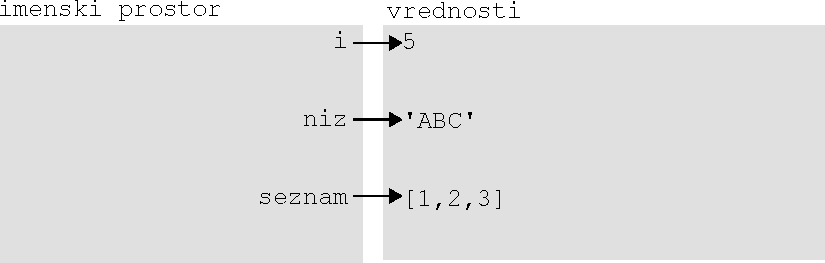
\includegraphics[width=\linewidth]{img/spremenljivost.pdf}
    \caption{Ob prireditvi se imenu spremenljivke priredi podana vrednost.}
    \label{img:spremenljivost}
\end{figure}
Kaj pa se zgodi, če spremenljivko priredimo drugi spremenljivki, na primer takole:
\begin{lstlisting}[language=Python, showstringspaces=false]
>>> i = 1
>>> j = i
>>> niz1 = 'ABC'
>>> niz2 = niz1
>>> seznam1 = [1,2,3]
>>> seznam2 = seznam1
\end{lstlisting}
Nekaj podobnega smo srečali že pri klicu funkcije. Spomnimo se, da se v Pythonu v takem primeru naredi t.i. \textit{plitva kopija} spremenljivke. To pomeni, da vrednost v pomnilniku dobi novo ime. Do dejanskega (\textit{globokega}) kopiranja vrednosti v tem primeru ne pride. To lahko ponazorimo s sliko \ref{img:spremenljivost_2}.
\begin{figure}
    \centering
    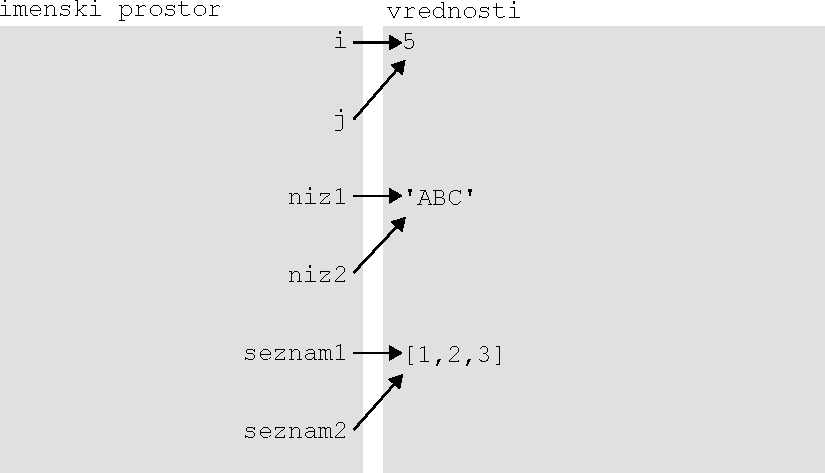
\includegraphics[width=\linewidth]{img/spremenljivost_2.pdf}
    \caption{Ob prireditvi spremenljivke drugi spremenljivki se ustvari plitva kopija spremenljivke.}
    \label{img:spremenljivost_2}
\end{figure}
Na tak način je delovanje tako s časovnega stališča (hitrost) kot tudi s prostorskega stališča (poraba pomnilnika) bolj varčno. 

\section{Kaj se zgodi ob spreminjanju vrednosti spremenljivk?}
Kaj pa se zgodi, če vrednost nove (ali pa stare) spremenljivke spremenimo? Vse skupaj zavisi od tega ali je podatek, ki ga spreminjamo spremenljiv ali ne. Spomnimo se. Spremenljiv podatek lahko spreminjamo, ko pa pokusimo spremeniti nespremenljiv podatek, se ustvari njegova kopija (globoka), ki odraža narejeno spremembo. Če npr. uporabimo operator \texttt{+=}, bo v primeru spremenljivega podatka spremenjen obstoječ podatek, v primeru nespremenljivega podatka pa bo ustvarjen nov podatek, ki bo odražal narejeno spremembno. 

Kaj pa se zgodi v primeru, da na podatek kaže več imen, kot v scenariju zgoraj. Ali se bo po izvedbi spodnje kode sprememba odražala tudi preko drugih imen podatka? Poglejmo si spodnjo kodo.
\begin{lstlisting}[language=Python, showstringspaces=false]
>>> i = 1
>>> j = i
>>> j += 1
>>> niz1 = 'ABC'
>>> niz2 = niz1
>>> niz2 += 'D'
>>> seznam1 = [1,2,3]
>>> seznam2 = seznam1
>>> seznam2 += [4]
\end{lstlisting}
Zanima nas ali se po spreminjanju spremenljivk \texttt{j}, \texttt{niz2} in \texttt{seznam2} spremembe odražajo tudi na spremenljivkah \texttt{i}, \textbf{niz1} in \texttt{seznam1}. Odgovor ni enostvane da ali ne. Odgovor je namreč odvisen od spremenljivosti podatka, ki ga spreminjamo. Situacijo po spreminjanju podatka z operatorjem \texttt{+=} prikazuje slika \ref{img:spremenljivost_3}.
\begin{figure}
    \centering
    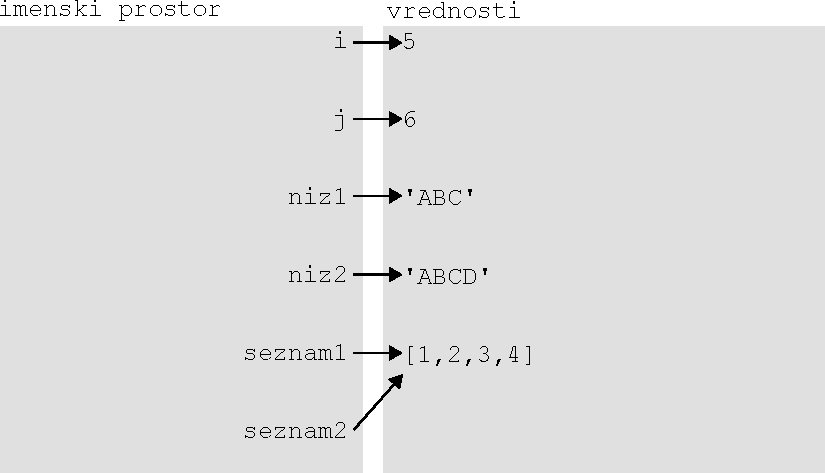
\includegraphics[width=\linewidth]{img/spremenljivost_3.pdf}
    \caption{Ob spreminjanju spremenljivih podatkov se spremenijo vse plitve kopije podatka.}
    \label{img:spremenljivost_3}
\end{figure}
V primeru, da je podatek spremenljiv, se torej sprememba odraža na vseh spremenljivkah, ki predstavljajo plitve kopije tega podatka. S tem ko v zgornjem zgledu spreminjamo spremenljivko \texttt{seznam2}, spreminjamo tudi spremenljivko \texttt{seznam1}. Po drugi strani spreminjanje spremenljivk \texttt{j} in \texttt{niz2} ustvari globoko kopijo spremenljivk \texttt{j} in \texttt{niz2}, ki odraža narejeno spremembo. Globoka kopija predstavlja nov podatek, tj. podatek ki se razlikuje od tistega, na katerega kažeta imeni \texttt{i} in \texttt{niz1}. Posledica tega je, da spreminjanje vrednosti spremenljivk \texttt{j} in \texttt{niz2} na vrednostih spremenljivk \texttt{i} in \texttt{niz1} ne vplivajo, saj pripadajo nespremenljivim podatkovnim tipom.

\section{Ali funkcije spreminjajo vrednosti svojim argumentom?}
Spomnimo se, da se ob klicu funkcije ustvari lokalni imenski prostor funkcije. V lokalnem imenskem prostoru se ob klicu spremenljivkam, ki nastopajo kot argumenti funkcije, priredijo vrednosti, s katerimi smo funkcijo poklicali. V primeru, da smo funkcijo poklicali z globalnimi spremenljivkami, se argumentom funkcije priredi plitva kopija teh spremenljivk. Vprašanje pa je ali se bodo ob spreminjanju argumentov funkcije spremembe odražale tudi izven funkcije, torej po tem, ko se bo funkcija že končala. Vprašanje lahko ponazorimo s spodnjim zgledom.

\begin{zgled}
Kakšna je vrednost spremenljivk \texttt{st1}, \texttt{niz1} in \texttt{seznam1} po izvedbi spodnje kode in kakšen bo izpis programa?
\begin{lstlisting}[language=Python, showstringspaces=false,numbers=left]
def spremeni(a, b):
    a += b

i = 1
j = 2
spremeni(i,j)
print(i)

niz1 = "ABC"
niz2 = "D"
spremeni(niz1,niz2)
print(niz1)

seznam1 = [1,2,3]
seznam2 = [4,5,6]
spremeni(seznam1,seznam2)
print(seznam1)
\end{lstlisting}
\end{zgled}

\begin{resitev}
Ob klicu funkcije spremenljivki, s katerima funkcijo pokličemo, dobita plitvi kopiji z imeni \texttt{a} in \texttt{b} v lokalnem imenskem prostoru funkcije. Znotraj funkcije plitvo kopijo z imenom \texttt{a} spreminjamo. V primeru, da je spremenljivka spremenljivega podatkovnega tipa (npr. seznam) se spreminja obstoječ podatek, na katerega kaže tudi globalna spremenljivka, kar pomeni, da se bo sprememba odražala tudi izven funkcije. V primeru, da je spremenljivka nespremenljivega podatkovnega tipa, se ustvari globoka kopija podatka, ki bo odražala narejeno spremembo. Spremeni se torej zgolj spremenljivka, ki je definirana znotraj funkcije, ta sprememba pa izven funkcije ne bo vidna. 

Spremenljivki \texttt{i} in \texttt{niz1} se torej po klicu funkcije ne bosta spremenili, spremenljivka \texttt{seznam1} pa se bo spremenila. Po izvedbi programa bo izpis sledeč:

\begin{lstlisting}[language=Python, showstringspaces=false]
1 # nespremenjena vrednost
ABC # nespremenjena vrednost
[1,2,3,4,5,6] # spremenjena vrednost
\end{lstlisting}

\end{resitev}

Funkcije torej lahko spreminjajo vrednosti svojim argumentom, tako da so spremembe vidne tudi izven funkcij, ampak samo v primeru, ko so podani argumenti spremenljivega podatkovnega tipa. 



\section{Terke}

Zdaj, ko vemo, kaj je to spremenljivost, lahko razložimo tudi, kaj so terke \angl{tuples}. Terka oziroma \texttt{tuple} predstavlja sekvenčen podatkovni tip, ki je nespremenljiv. Ker terke zelo spominjajo na sezname, bi jim lahko rekli tudi nespremenljivi seznami. Načeloma bi lahko pri programiranju shajali tudi brez njih (tako kot bi lahko shajali tudi brez zanke \texttt{for}), ampak njihova uporaba v veliko primerih naredi naše programe lepše in boljše (tako kot uporaba zanke \texttt{for}).

\section{Uporaba terk}

Terko definiramo z navadnimi oklepaji, tj. \texttt{(} in \texttt{)}, znotraj katerih naštejemo elemente. Terko treh elementov, bi lahko definirali na primer takole:
\begin{lstlisting}[language=Python, showstringspaces=false]
>>> terka=("Janez", 1.8, 75)
\end{lstlisting}
Za terko je pa mogoče bolj kot oklepaji bistveno naštevanje elementov, zato bi tudi, če bi oklepaje izpustili, dobili terko. Takole:
\begin{lstlisting}[language=Python, showstringspaces=false]
>>> terka="Janez", 1.8, 75
>>> terka
("Janez", 1.8, 75)
>>> type(terka)
<class 'tuple'>
\end{lstlisting}
Python je ob naštevanju elementov z vejicami ugotovil, da želimo imeti terko in jo naredil. Python ima nekoliko težav, ko želimo narediti terko dolžine 1, saj si v tem primeru oklepaje razlaga kot operator, ki določa prioriteto. V primeru, da znotraj oklepajev damo zgolj eno npr. celo število, bomo torej dobili podatek, ki pripada podatkovnemu tipu \texttt{int} in ne \texttt{tuple}:
\begin{lstlisting}[language=Python, showstringspaces=false]
>>> terka=(1)
>>> terka
1
>>> type(terka)
<class 'int'>
\end{lstlisting}
Že prej smo omenili to, da je bistvena lasntnost terk naštevanje elementov, ki jih ločimo z vejicami. Kako v primeru enega elementa povemo, da gre za naštevanje? Tako, da za njim napišemo vejico:
\texttt{tuple}:
\begin{lstlisting}[language=Python, showstringspaces=false]
>>> terka=(1,)
>>> terka
(1,)
>>> type(terka)
<class 'tuple'>
\end{lstlisting}
Gre pa seveda tudi brez oklepajev:
\texttt{tuple}:
\begin{lstlisting}[language=Python, showstringspaces=false]
>>> terka=1,
>>> terka
(1,)
>>> type(terka)
<class 'tuple'>
\end{lstlisting}

Kaj lahko s terkami počnemo? Podobno kot sezname lahko elemente terke indeksiramo, lahko delamo rezine, lahko preverjamo vsebovanost elementov, z zanko \texttt{for} se lahko čez elemente terke sprehajamo itd. Z njimi lahko delamo torej skoraj vse, kar smo delali s seznami. Skoraj vse? Ker so terke nespremenljive, jih seveda ne moremo spreminjati, tako kot lahko spreminjamo sezname. Poskusimo:
\begin{lstlisting}[language=Python, showstringspaces=false]
>>> terka = ("Janez", 1.8, 75)
>>> terka[0] = "Marko"
Traceback (most recent call last):
  File "<pyshell#6>", line 1, in <module>
    terka[0] = "Marko"
TypeError: 'tuple' object does not support item assignment
\end{lstlisting}
Očitno res ne gre. Seveda ne, saj so nespremenljive. Zakaj bi terke potem sploh uporabljali? Nekaj primerov, pri katerih je uporaba terk smiselna, je podanih v nadaljevanju poglavja.

\section{Seznami terk in razpakiranje elementov terk}

Nenapisano pravilo (ki ga seveda lahko kršimo) je, da v sezname shranjujemo homogene podatke, torej podatke, ki se nanašajo npr. na isto spremenljivko. To pomeni, da vsak element seznama obravnavamo na enak način, saj se nanaša na isto količino. Terke se pogosto uporabljajo za shranjevanje heterogenih podatkov, tj. podatkov različnih tipov, ki pa pripadajo isti entiteti, kot je npr. oseba ali meritev. Če si torej želimo pri določeni entiteti zabeležiti več podatkov, lahko uporabimo seznam terk. Na primer, če imamo vzorec oseb, pri čemer za vsako osebo beležimo ime, višino in težo, potem lahko uporabimo seznam terk, pri čemer vsaka izmed terk vsebuje ime, višino in težo dotične osebe. Primer takega seznama bi bil
\begin{lstlisting}[language=Python, showstringspaces=false]
meritve = [("Janez", 1.8, 75),
           ("Ana", 1.65, 60), 
           ("Nika", 1.66, 55)]
\end{lstlisting}
Elementi seznama so torej homogeni, kar pomeni, da bomo vsakega obravavali enako. Elementi seznama so namreč terke, ki imajo vsakič enako obliko. Na 0-tem indeksu je shranjeno ime osebe, na indeksu 1 višina v metrih in na indeksu 2 teža osebe v kilogramih. Elementi posamezne terke pa očitno pripadajo različnim spremenljivkam.

Tak način predstavitve podatkov bomo srečali velikokrat. Kako pa lahko tako shranjene podatke uporabimo pri nadaljnji analizi. Na primer pri izračunu in izpisu indeksa telesnih mas posamezne osebe v seznamu. Tako, da se čez seznam sprehodimo z zanko \texttt{for} in v vsaki iteraciji zanke tekočo terko \emph{razpakiramo} in tako pridemo do konkretnih vrednosti. To lahko naredimo na sledeč način: 
\begin{lstlisting}[language=Python, showstringspaces=false]
for meritev in meritve:
    ime = meritev[0]
    visina = meritev[1]
    teza = meritev[2]
    itm = teza/visina**2
    print("ITM osebe", ime, "je", itm)
\end{lstlisting}
Do posameznih elementov terke smo torej prišli z njihovim indeksiranjem. Terke pa lahko razpakiramo veliko hitreje, in sicer tako, da terko priredimo drugi terki, ki vsebuje imena spremenljivk, v katere želimo vrednosti shraniti oziroma razpakirati. Takole:
\begin{lstlisting}[language=Python, showstringspaces=false]
(spremenljivka1, spremenljivka2,...) = terka
\end{lstlisting}
Paziti moramo le na to, da terka na levi strani vsebuje enako število elementov kot terka na desni strani prireditvenega stavka. Kaj smo v zgornjem stavku pravzaprav naredili? Naredili smo terko spremenljivk, ki smo ji priredili terko na desni strani. Ker terki spremenljivk nismo dali nobenega imena, je v imenski prostor nismo shranili in zato tudi ni shranjena nikjer v pomnilniku. So pa v pomnilniku ostale spremenljivke, v katere smo razpakirali terko na desni. Kot smo videli že zgoraj pa lahko oklepaje pri definiciji tudi izpustimo. Torej lahko napišemo tudi nekaj takega
\begin{lstlisting}[language=Python, showstringspaces=false]
spremenljivka1, spremenljivka2,... = terka
\end{lstlisting}
Mimogrede, tako razpakiranje elementov bi delovalo tudi, če bi imeli na desni strani prireditvnega stavka seznam.

Tak način razpakiranja elementov lahko uporabimo v našem zgledu z računanjem indeksa telesnih mas, s čimer se koda občutna skrajša:
\begin{lstlisting}[language=Python, showstringspaces=false]
for meritev in meritve:
    ime, visina, teza = meritev
    itm = teza/visina**2
    print("ITM osebe", ime, "je", itm)
\end{lstlisting}
Kodo lahko še dodatno skrajšamo, če razpakiranje naredimo kar v glavi zanke \texttt{for}:
\begin{lstlisting}[language=Python, showstringspaces=false]
for ime, visina, teza in meritve:
    itm = teza/visina**2
    print("ITM osebe", ime, "je", itm)
\end{lstlisting}

\section{Pakiranje seznamov v sezname terk}
Seznami terk, kot smo jih srečali zgoraj, torej predstavljajo lep način zapisovanja podatkov, ko želimo pri posamezni entiteti imeti več podatkov. Dejstvo pa je, da velikokrat podatkov ne dobimo v taki obliki, ampak dobimo za vsako količino svoj seznam. Pri tem so seznami med seboj poravnani, kar pomeni, da istoležni elementi v vseh seznamih pripadajo isti entiteti. Elementi na indeksu 0 torej pripadajo entiteti 0, elementi na indeksu 1 entiteti 1 itd. V primeru imen, višin in tež, bi torej imeli tri sezname v obliki 
\begin{lstlisting}[language=Python, showstringspaces=false]
imena = ["Janez", "Ana", "Nika"]
visine = [1.8, 1.65, 1.66]
teze = [75, 60, 55]
\end{lstlisting}
Elementi vseh treh seznamov torej na indeksu 0 pripadajo Janezu, na indeksu 1 Ani in na indeksu 2 Niki. Kaj imajo ti seznami skupnega? Indekse! Čez take podatke bi se torej lahko sprehodili tako, da se sprehajamo po indeksih in ne direktno po elementih. Naredimo torej sprehod z znako \texttt{for} od indeksa 0 do dolžine seznama - 1. Dolžine katerega seznama? Ni važno, saj so vsi enko dolgi (oziroma vsaj smiselno bi bilo, da so). To bi lahko naredili takole:  
\begin{lstlisting}[language=Python, showstringspaces=false]
for i in range(len(imena)):
    ime = imena[i]
    visina = visine[i]
    teza = teze[i]
    itm = teza/visina**2
    print("ITM osebe", ime, "je", itm)
\end{lstlisting}
Kako pa bi lahko iz treh seznamov naredili seznam terk, s katerim smo delali zgoraj. Izkaže se, da se s takim problemom srečamo relativno pogosto, zato nam Python za \emph{zapakiranje} več seznamov v seznam terk ponuja vgrajeno funkcijo \texttt{zip}. Funkcija \texttt{zip} iz zgornjih treh seznamov naredi točno to, kar bi si želeli: 
\begin{lstlisting}[language=Python, showstringspaces=false]
>>> meritve = zip(imena, visine, teze)
>>> meritve
<zip object at 0x0000019A2A865D48>
\end{lstlisting}
Tale izpis je malo čuden, ampak ni z njim nič narobe. Funkcija \texttt{zip} je t.i. \emph{iterator}, ki dejanski seznam elementov vrne, šele ko ga potrebujemo oziroma posamezne elemente seznama vrača sproti. Če bi želeli imeti lepši izpis, bi lahko do njega prišli tako, da rezultat funkcije \texttt{zip} eksplicitno pretvorimo v seznam s funkcijo \texttt{list}:
\begin{lstlisting}[language=Python, showstringspaces=false]
>>> meritve = list(zip(imena, visine, teze))
>>> meritve
[('Janez', 1.8, 75), ('Ana', 1.65, 60), ('Nika', 1.66, 55)]
\end{lstlisting}
Sprehod čez sezname lahko torej naredimo na podoben način kot v prejšnjem poglavju, le da prej sezname zapakiramo v seznam terk:
\begin{lstlisting}[language=Python, showstringspaces=false]
for ime, visina, teza in zip(imena, visine, teze):
    itm = teza/visina**2
    print("ITM osebe", ime, "je", itm)
\end{lstlisting}

\section{Zahteva po nespremenljivosti}
V določenih primerih Python zahteva uporabo nespremenljivih podatkovnih tipov. Nespremenljive podatkovne tipe moramo uporabiti, kadar želimo podatke shranjevati v množico (\texttt{set}) in kadar želimo nek podatek uporabiti kot ključ (\texttt{key}) slovarja (\texttt{dict}). Če želimo v takem primeru uporabiti več elementov, moramo namesto po seznamu poseči po terki. V teh primerih je torej uporaba terk obvezna. Več o množicah in slovarjih bomo izvedeli prav kmalu.

Drug primer, v katerem bi nespremenljivost bila zaželena (ne pa obvezna), je, ko ne želimo, da funkcija spremeni vrednosti posanega argumenta. Kot smo videli lahko funkcije spreminjajo vrednosti svojih argumentov, tako da bodo spremembe vidne tudi izven funkcij. Če bi radi zagotovilo, da se podan argument izven funkcije zagotovo ne bo spremenil, namesto spremenljivega seznama enostavno uporabimo nespremenljivo terko. V tem kontekstu si poglejmo spodnji zgled.

\begin{zgled}
Kakšna je vrednost spremenljivk \texttt{seznam1} in \texttt{terka1}  po izvedbi spodnje kode in kakšen bo izpis programa?
\begin{lstlisting}[language=Python, showstringspaces=false,numbers=left]
def spremeni(a, b):
    a += b

seznam1 = [1,2,3]
seznam2 = [4,5,6]
spremeni(seznam1,seznam2)
print(seznam1)

terka1 = (1,2,3)
terka2 = (4,5,6)
spremeni(terka1,terka2)
print(terka1)
\end{lstlisting}
\end{zgled}

\begin{resitev}
Kot smo videli že prej, se sprememba, ki smo jo nad plitvo kopijo spremenljivke \texttt{seznam1} naredili znotraj funkcije, odraža tudi izven funkcije, saj je seznam spremenljiv podatkovni tip. Ko torej spreminjamo njegovo plitvo kopijo, s tem spreminjamo vse spremenljivke, ki nanj kažejo. 

Kaj pa se zgodi, ko funkcijo pokličemo s terko. Najprej se ustvari plitva kopija terke v lokalnem imenskem prostoru funkcije (spremenljivka \texttt{a}). Ker je terka nespremenljiv podatkovni tip, je ne moremo spreminjati. Ob njenem spreminjau se zato ustvari globoka kopija, torej nov podatek v pomnilniku, ki odraža narejeno spremembo. Na ta podatek pa kaže zgolj lokalna spremenljivka \texttt{a}. Ko se funkcija zaključi, njen lokalni imenski prostor skupaj z lokalno spremenljivko \texttt{a} izgine (tako kot tudi spremenjena terka -- globoka kopija terke, s katero smo funkcijo poklicali). V sled temu sprememba, ki smo jo naredili znotraj funkcije, izven funkcije ni vidna.

Po izvedbi funkcije \texttt{spremeni} ima spremenljivka \texttt{seznam1} spremenjeno vrednost (\texttt{[1,2,3,4,5,6]}), spremenljivka \texttt{terka1} pa ostane taka, kot je bila pred klicem funkcije (\texttt{(1,2,3)}). Izpis programa je torej
\begin{lstlisting}[language=Python, showstringspaces=false]
[1,2,3,4,5,6] # spremenjena vrednost
(1,2,3) # nespremenjena vrednost
\end{lstlisting}

\end{resitev}

Funkcijam, ki kot argumente sprejemajo spremenljive podatkovne tipe, spremenjenih vhodnih argumentov ni potrebno vračati, saj se bodo spremembe odražale tudi izven funkcije. Funkcije, ki kot argumente sprejemajo nespremenljive podatkovne tipe, morajo spremenjene vhodne argumente eksplicitno vrniti, saj so spremenjene vrednosti sicer za vedno izgubljene. Oba načina si poglejmo v spodnjih zgledih.

Najprej si poglejmo kako se lotiti pisanja in uporabe funkcije, ki sprejema nespremenljive podatke.
\begin{zgled}
Napiši funkcijo \texttt{dodaj\_AT\_niz}, ki sprejme dve nukleotidini zaporedji zapisani kot niza in v prvo zaporedje doda vse ponovitve baz \texttt{A} in \texttt{T} v enakem zaporedju kot nastopajo v drugem nizu. Funkcijo uporabi na zaporedjih \texttt{'ATCG'} in \texttt{'AATGGAATGG'}, tako da bo prvo zaporedje po njeni izvedbi spremenjeno.
\end{zgled}

\begin{resitev}
Funkcija sprejema in spreminja podatke tipa \texttt{str}, ki je nespremenljiv podatkovni tip. Če bomo vhodne argumente spreminjali znotraj funkcije, se te spremembe izven funkcije ne bodo odražale, kar pomeni, da mora funkcija vračati spremenjen niz. Napišimo jo.
\begin{lstlisting}[language=Python, showstringspaces=false]
def dodaj_AT_niz(zaporedje1, zaporedje2):
    for baza in zaporedje2:
        if baza in 'AT':
            zaporedje1 += baza
    return zaporedje1
\end{lstlisting}
Na koncu torej vrnemo spremenjeno zaporedje1. Kljub temu, da smo znotraj funkcije to spremenljivko spreminjali, spremembe izven funkcije ne bodo vidne.

Klic funkcije moramo izvesti na tak način, da bo spremenila vrednost prve spremenljive, s katero funkcijo kličemo. Kako to doseči? Enostavno tako, da rezultat funkcije priredimo vrednosti te spremenljivke. Takole:
\begin{lstlisting}[language=Python, showstringspaces=false]
>>> zaporedje1 = 'ATCG'
>>> zaporedje2 = 'AATGGAATGG'
>>> zaporedje1 = dodaj_AT_niz(zaporedje1, zaporedje2)
\end{lstlisting}
Na tak način smo vrednost spremenljivke \texttt{zaporedje1} spremenili.
\end{resitev}

Poglejmo si še kakšne so razlike pri delu s spremenljivimi podatki.
\begin{zgled}
Napiši funkcijo \texttt{dodaj\_AT\_seznam}, ki sprejme dve nukleotidini zaporedji zapisani kot seznama enoznakovnih nizov (baz) in v prvo zaporedje doda vse ponovitve baz \texttt{A} in \texttt{T} v enakem zaporedju kot nastopajo v drugem nizu. Funkcijo uporabi na zaporedjih \texttt{['A','T','C','G']} in \texttt{'A','A','T','G','G','A','A','T','G','G'}, tako da bo prvo zaporedje po njeni izvedbi spremenjeno.
\end{zgled}
\begin{resitev}
Navodilo naloge je praktično enako kot prej, le da tokrat namesto nespremenljivih podatkovnih tipov uporabljamo spremenljive. To pomeni, da ni potrebe po tem, da funkcija vrača spremenjen rezultat, saj se bodo spremembe odražale že preko podanega argumenta. Koda je torej sledeča:
\begin{lstlisting}[language=Python, showstringspaces=false]
def dodaj_AT_seznam(zaporedje1, zaporedje2):
    for baza in zaporedje2:
        if baza in 'AT':
            zaporedje1.append(baza)
\end{lstlisting}
Tokrat funkcija ne vrača ničesar uporabnega, zato njenega rezultata nima smisla ničemur prirejati. Vse kar potrebujemo je klic funkcije z ustreznimi argumenti:
\begin{lstlisting}[language=Python, showstringspaces=false]
>>> zaporedje1 = ['A','T','C','G']
>>> zaporedje2 = ['A','A','T','G','G','A','A','T','G','G']
>>> dodaj_AT_seznam(zaporedje1, zaporedje2) 
\end{lstlisting}
Prepričajmo se, če je vrednost spremenljivke \texttt{zaporedje1} res spremenjena:
\begin{lstlisting}[language=Python, showstringspaces=false]
>>> zaporedje1
['A', 'T', 'C', 'G', 'A', 'A', 'T', 'A', 'A', 'T']
\end{lstlisting}




\end{resitev}